% file siminos/froehlich/slice/slice.tex
% $Author$ $Date$

% \section{Dynamics in the slice}
% \section{\Mslices} % OLD
%       \label{sec:mslices}



Any \statesp\ trajectory can be written in a factorized
form $\ssp(\tau)=\LieEl(\tau)
\sspRed(\tau)$. Differentiating both sides with respect to time and
setting $\velRed={d\sspRed}/{d\tau}$ we find
\(
\vel(\ssp)=\dot{\LieEl} \, \sspRed+\LieEl \, \velRed(\sspRed)
\,.
\)
By the equivariance \refeq{eq:FiniteRot}
\[
\vel=\velRed + \LieEl^{-1} \, \dot{\LieEl} \, \sspRed
\,.
\]
Noting that $\LieEl^{-1}\dot{\LieEl}=e^{-\gSpace \cdot \Lg} \,
\frac{d ~~}{d \, \tau} e^{\gSpace \cdot \Lg}=\dot{\gSpace}\cdot \Lg$,
we obtain the equation for the velocity of the reduced flow:
\beq
\velRed(\sspRed)=\vel(\sspRed)-\dot{\gSpace}(\sspRed)\cdot \groupTan(\sspRed).
\ee{eq:redVel}
In other words, the velocity in the full \statesp\ is the sum of the
velocity normal along the group tangent and the remainder $\velRed$.

This equation is true for any factorization $\ssp(\tau)=\LieEl(\tau)
\sspRed(\tau)$, and by itself provides no information on how to calculate
$\dot{\gSpace}$. Let
$\sliceTan{a}$ be the group tangents at the slice
fixing point. Requirement \refeq{PCsectQ0} that the flow is confined to the slice,
yields
\beq
\braket{\vel(\sspRed)}{\sliceTan{a}}
 -\braket{\dot{\gSpace}\cdot \groupTan(\sspRed)}{\sliceTan{a}}=0
\,.
\label{eq:slicecondition}
\eeq
% for each group tangent $\sliceTan{a}$ at the slice fixing point.
In principle\rf{FiSaScWu96} this is a matrix equation in
$\braket{\groupTan_b(\sspRed)}{\sliceTan{a}}$ that one can solve
for $\dot{\gSpace}_a$. Here we shall consider only the
$\SOn{2}$ case, which has a single group tangent:
\bea
\velRed(\sspRed) &=& \vel(\sspRed)
   -\dot{\gSpace}(\sspRed) \groupTan(\sspRed)
\continue
\dot{\gSpace}(\sspRed) &=& {\braket{\vel(\sspRed)}{\sliceTan{}}}/
               {\braket{\groupTan(\sspRed)}{\sliceTan{}}}
\,.
\label{eq:so2reduced}
\eea
The first equation defines the flow confined to the slice
(see \reffig{fig:RedTrajNoPlane1}), and
integration of the second, `reconstruction'
equation\rf{Marsd92,MarsdRat94} enables us to reconstruct the
corresponding trajectory in the full \statesp.
%\item[2010-12-06 PC] in Siminos blog
Perhaps the insightful way to think about reduction of a flow to a slice
is in terms of Lagrange multipliers (see {Stone and Goldbart}\rf{StGo09},
Sect 1.5 for intuitive, geometrical interpretation of Lagrange multipliers).

% Former {CLEreduced}
 \begin{figure}
 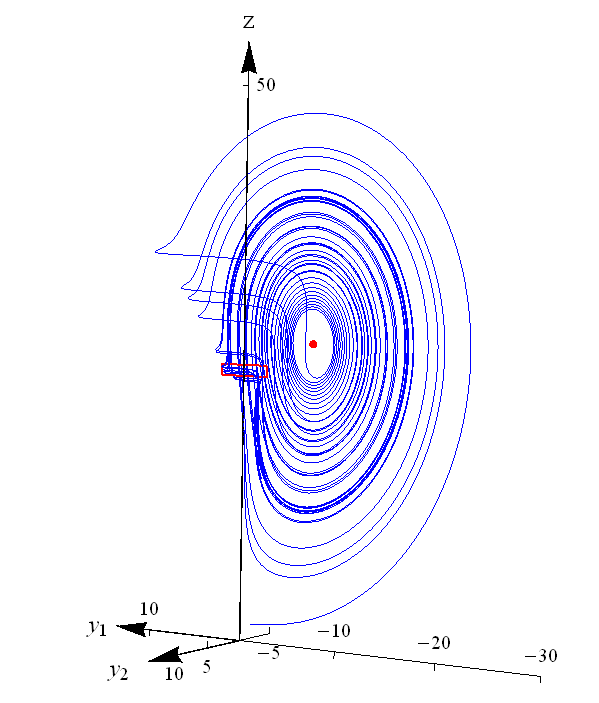
\includegraphics[width=0.35\textwidth]{RedTrajNoPlane1}%
 \caption{\label{fig:RedTrajNoPlane1}
A $\{y_1,y_2,z\}$ plot of the \reducedsp\ \cLf\ strange attractor
with initial point
%$(x_1, x_2, y_1, y_2, z) = (1, 2, 3, 1, 2)$
in the
slice normal to $\sliceTan{}=(1,0,0,0,0)$. Contrast this plot with
\reffig{fig:Fullspace}, and note the semicircular jumps in the
reduced flow. For a blow-up of such jump, see \reffig{fig:singpass}.
 }%
 \end{figure}

%
% ****** End of file slice.tex ******
